\documentclass[letterpaper, 12pt]{report}
\usepackage[utf8]{inputenc}
\usepackage{amsmath,amssymb,amsthm}
\usepackage[spanish]{babel}
\usepackage{graphicx}
\usepackage{caption}
\usepackage{subcaption}
\usepackage{xcolor}
\usepackage{titlesec}
\usepackage{lmodern}
\usepackage{fancyhdr}
\usepackage{geometry}
\usepackage{algorithm}
\usepackage{algpseudocode}
\usepackage{multirow}
\usepackage{booktabs}
\usepackage{listings}
\usepackage{enumitem}

% Paradoja de pooling

\definecolor{codegreen}{rgb}{0,0.6,0}
\definecolor{codegray}{rgb}{0.5,0.5,0.5}
\definecolor{codepurple}{rgb}{0.58,0,0.82}

% \lstdefinestyle{mystyle}{
%     commentstyle=\color{codegreen},
%     keywordstyle=\color{magenta},
%     numberstyle=\tiny\color{codegray},
%     stringstyle=\color{codepurple},
%     basicstyle=\ttfamily\footnotesize,
%     breakatwhitespace=false,         
%     breaklines=true,                 
%     captionpos=b,                    
%     keepspaces=true,                 
%     numbers=left,                    
%     numbersep=5pt,                  
%     showspaces=false,                
%     showstringspaces=false,
%     showtabs=false,                  
%     tabsize=2,
%     frame=single
% }

%\lstset{style=mystyle}

\setlength{\headheight}{24.01996pt}
\addtolength{\topmargin}{-12.01996pt}

% Definir colores personalizados
\definecolor{primary}{RGB}{25,55,95}
\definecolor{secondary}{RGB}{200,35,45}

% Configurar márgenes
\geometry{
    left=3cm,
    right=2.5cm,
    top=3cm,
    bottom=2.5cm
}

\newtheorem*{theorem*}{Teorema}

% Configurar estilo de títulos
\titleformat{\chapter}[display]
{\normalfont\Huge\bfseries\color{primary}}
{\chaptertitlename\ \thechapter}{20pt}{\Huge}

\titleformat{\section}
{\normalfont\Large\bfseries\color{primary}}
{\thesection}{1em}{}

% Configurar encabezado y pie de página
\pagestyle{fancy}
\fancyhf{}
\fancyhead[L]{\small\textcolor{primary}{\nouppercase{\leftmark}}}
\fancyfoot[C]{\textcolor{primary}{\thepage}}
\renewcommand{\headrulewidth}{0.4pt}
\renewcommand{\headrule}{\hbox to\headwidth{\color{primary}\leaders\hrule height \headrulewidth\hfill}}

% Portada personalizada
\newcommand*{\customtitlepage}{
    \begin{titlepage}
        \begin{center}
            \vspace*{1cm}
            
            
            {\LARGE \textbf{UNIVERSIDAD DE LA HABANA}}\\
            \vspace{0.5cm}
            {\Large Facultad de Matem\'atica y Computaci\'on}\\
            

            
\includegraphics[scale=0.5]{images/logo.png}
            
            \vspace{1cm}
            
            
            \rule{\textwidth}{1.5pt}\\
            \vspace{0.5cm}
            {\LARGE \textcolor{primary}{\textbf{Primer Proyecto de Simulación}}}
            \vspace{0.5cm}
            \rule{\textwidth}{1.5pt}
            
            \vspace{2cm}
            
            {\Large \textbf{Servidores Especializados vs Servidores Generalistas}}\\
            \vspace{1cm}
            
            {\Large \textbf{Autor:} Lidier Robaina Caraballo \\
            \vspace{0.5cm}
            {\Large \textbf{Grupo:} C-411 }\\
            \vspace{1.5cm}
            
            {\Large 13 de abril de 2025
            }
            }
        \end{center}
    \end{titlepage}
}

\begin{document}

\customtitlepage

% Índice
\tableofcontents
\thispagestyle{empty}
\cleardoublepage

% Contenido principal
\setcounter{page}{1}

\chapter{Introducción}


En el ámbito de la gestión de servicios, la elección entre estrategias especializadas o generalistas representa 
un dilema recurrente, donde la eficiencia operativa y la experiencia del usuario dependen de la configuración 
de los recursos disponibles. Este proyecto aborda dicho desafío mediante la simulación computacional 
basada en eventos discretos, un enfoque que permite modelar sistemas dinámicos bajo condiciones
controladas. \\

El estudio se centra en comparar dos escenarios: uno con servidores dedicados a tareas específicas
(estrategia especializada) y otro en el que los servidores son flexibles y pueden atender múltiples tipos
de demandas (estrategia generalista). Aunque el análisis se contextualiza en un caso sencillo de una sucursal bancaria,
los resultados se orientan a ofrecer conocimientos aplicables a sistemas de servicios más amplios y complejos.

\section{Objetivos y metas}
El proyecto tiene como objetivo principal analizar y comparar el desempeño de las dos configuraciones operativas mencionadas anteriormente. Para ello, se definen las siguientes metas:

\begin{itemize}
    \item[1.] Calcular la eficiencia global de cada estrategia, cuantificando métricas clave como: congestión del sistema, tiempo de espera del usuario, 
    probabilidad de retrasos críticos y subutilización de recursos.  
    \item[2.] Evaluar trade-off entre la flexibilidad operativa (capacidad de atender múltiples tareas) y la velocidad de servicio, considerando posibles incrementos en los tiempos de atención al adoptar una estrategia generalista.
    \item[3.] Proporcionar recomendaciones basadas en datos para la optimización de sistemas de servicios, extrapolables a contextos como logística, atención al cliente o salud.
\end{itemize}

\newpage

\section{Sistema específico a simular}

\begin{quote}
    Una pequeña sucursal de un banco tiene dos empleados, uno para los pagos y otro para los cobros. Los clientes llegan a 
cada caja siguiendo una distribución de Poisson con una media de 20/hora (el total de llegada al banco es de 40/hora). 
El tiempo de servicio de cada empleado es una negativa exponencial de media 2 minutos. El encargado de la sección está 
pensando hacer un cambio en que los dos operarios puedan hacer tanto pagos como cobros para evitar situaciones en que 
una cola está llena y la otra parada. Sin embargo, se estima que cuando los empleados se encarguen de las dos cosas 
el tiempo de servicio aumentará a una media de 2,4 minutos. Compara el sistema que se emplea ahora con el propuesto, 
calculando el total de gente en el banco, el tiempo medio que pasaría un cliente en el banco hasta que es atendido, 
la probabilidad de que un cliente espere más de cinco minutos y el tiempo medio que están parados los empleados. \footnote{Problema 6.5 de \cite{queue}}
\end{quote}

De la definición del problema se obtienen las siguientes variables de interés:
\begin{itemize}
    \item \textbf{L:} Media del total de clientes en el sistema en cada instante (congestión del sistema)
    \item \(\mathbf{W_q}\)\textbf{:} Media del tiempo durante el que un cliente permanece en la cola (tiempo de espera)
    \item \(\mathbf{P ( W_q > t_k)}\)\textbf{:} Probabilidad de que el tiempo de espera sea superior a un tiempo determinado (retrasos críticos)
    \item \(\mathbf{t_{free}}\)\textbf{:} Media del tiempo durante el cual los servidores no tienen clientes (subutilización de recursos)  
\end{itemize}


\section{Variables que describen el problema}

\begin{itemize}
    \item \(\mathbf{\lambda_1}\)\textbf{:} tasa de llegadas de clientes para pagos (distribución Poisson con media $\lambda_1$)
    \item \(\mathbf{\lambda_2}\)\textbf{:} tasa de llegadas de clientes para cobros (distribución Poisson con media $\lambda_2$)    
    \item \(\mathbf{t_1}\)\textbf{:} tiempo de atención en el servidor 1 (distribución exponencial con media $t_1$)
    \item \(\mathbf{t_2}\)\textbf{:} tiempo de atención en el servidor 2 (distribución exponencial con media $t_2$)
    \item \textbf{s:} estrategia especializada vs generalista (variable categórica)
    \item \(\mathbf{t_k}\)\textbf{:} tiempo de espera crítico 
\end{itemize}

En caso de estrategia especializada, el servidor 1 atiende los pagos y el servidor 2 los cobros. En caso de estrategia generalista, $t_1 = t_2$.



\chapter{Implementación}

\section{Detalles de implementación}


\begin{itemize}
    \item[\textbf{1.}] \textbf{Gestión de Eventos:}
    Se emplea una cola de prioridad (módulo \texttt{heapq}) para manejar la lista cronológica de eventos. Cada evento contiene:
    \begin{itemize}
        \item Marca temporal de ejecución
        \item Tipo (llegada o salida)
        \item Metadatos específicos (índice de servidor/cola)
    \end{itemize}
    
    \item[\textbf{2.}] \textbf{Estructuras de Datos:}
    \begin{itemize}
        \item \textbf{Colas de espera}: Arreglos separados para cada servicio en modo especializado vs cola única compartida en modo generalista
        \item \textbf{Estado de servidores}: Arreglo booleano que indica disponibilidad
        \item \textbf{Contadores de clientes}: Registro separado por colas (especializado) o contador único (generalista)
    \end{itemize}
    
    \item[\textbf{3.}] \textbf{Mecánica de Simulación:}
    \begin{itemize}
        \item \textbf{Llegadas}: Generadas mediante proceso Poisson usando \texttt{random.expovariate()}
        \item \textbf{Tiempos de servicio}: Modelados con distribución exponencial negativa
        \item \textbf{Asignación de servidores}: Política FIFO con prioridad a servidores disponibles
    \end{itemize}
    
    \item[\textbf{4.}] \textbf{Recolección de Métricas:}
    \begin{itemize}
        \item \textit{Área acumulativa} para cálculos promediados en el tiempo
        \item Lista de tiempos de espera individuales
        \item Registro de ocupación de servidores
        \item Cálculo final mediante integración temporal (método de área bajo la curva)
    \end{itemize}
\end{itemize}

\section{Pasos de la simulación}


El flujo de ejecución sigue esta secuencia lógica:

\begin{enumerate}[leftmargin=1.5cm]
    \item \textbf{Inicialización:}
    \begin{itemize}
        \item Crear estructura de colas según estrategia
        \item Programar primeros eventos de llegada usando tasas $\lambda_1$ y $\lambda_2$
        \item Inicializar contadores y registros estadísticos
    \end{itemize}
    
    \item \textbf{Bucle Principal de Eventos:}
    \begin{lstlisting}[language=Python]
    while time < sim_time:
        event = heappop(events)
        actualizar_estadisticas()
        procesar_evento(event)
    \end{lstlisting}
    
    \item \textbf{Procesamiento de Llegadas:}
    \begin{itemize}
        \item Insertar cliente en la cola correspondiente
        \item Si hay servidor disponible:
        \begin{itemize}
            \item Iniciar servicio inmediato
            \item Registrar tiempo de espera cero
            \item Programar evento de salida
        \end{itemize}
        \item Generar próxima llegada según distribución Poisson
    \end{itemize}
    
    \item \textbf{Manejo de Salidas:}
    \begin{itemize}
        \item Liberar servidor
        \item Si existen clientes en cola:
        \begin{itemize}
            \item Extraer siguiente cliente
            \item Calcular tiempo de espera (current\_time - arrival\_time)
            \item Programar nuevo evento de salida
        \end{itemize}
    \end{itemize}
    
    \item \textbf{Actualización Estadística:}
    \begin{itemize}
        \item Calcular tiempo transcurrido desde último evento
        \item Acumular:
        \begin{itemize}
            \item Clientes-tiempo en sistema
            \item Tiempo ocupado de servidores
        \end{itemize}
        \item Mantener precisión temporal mediante integración continua
    \end{itemize}
    

\end{enumerate}

\chapter{Resultados y experimentos}

\section{Variables de interés}

Se ejecutaron 1000 simulaciones independientes para cada configuración del sistema. Para cada métrica, se comparan las distribuciones resultantes de ambas estrategias mediante el histograma normalizado y la distribución normal correspondiente a la media y desviación estándar de los datos.

\subsection{Análisis exploratorio}

\begin{figure}[H]
    \centering
    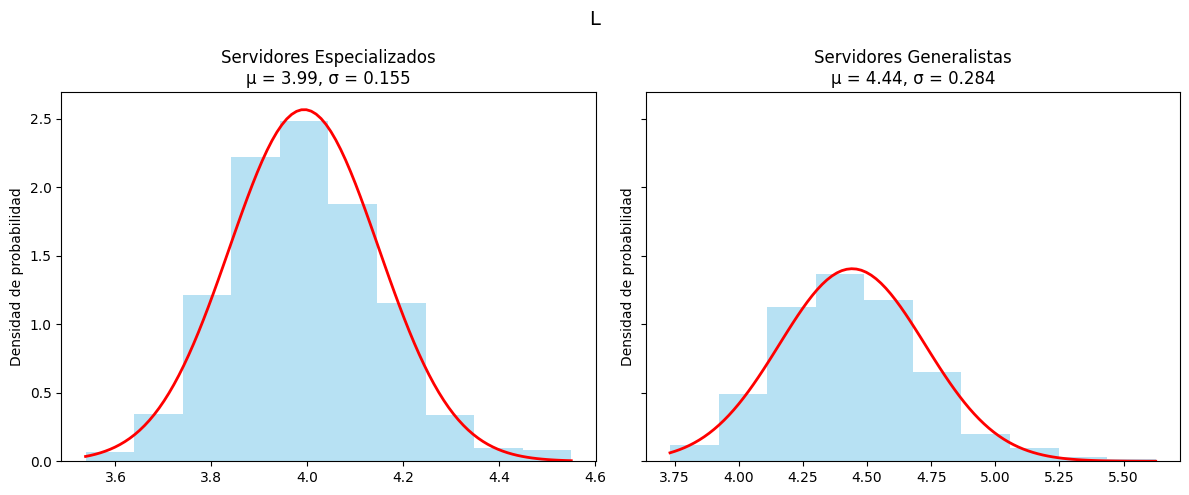
\includegraphics[width=0.95\textwidth]{images/L.png}
    \caption{Histograma de la media de clientes en el sistema ($L$)}
    \label{fig:clientes}
\end{figure}


\begin{figure}[H]
    \centering
    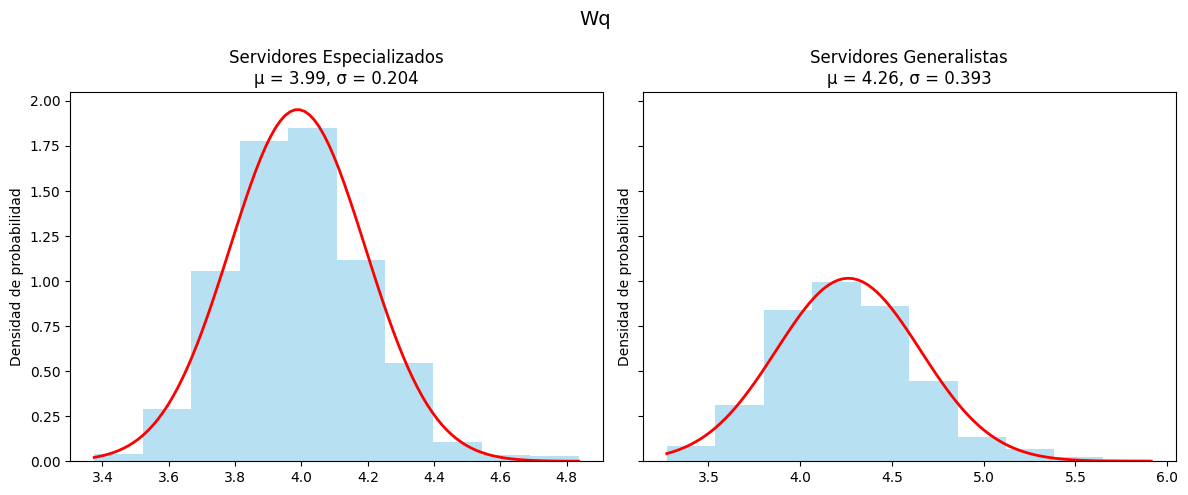
\includegraphics[width=0.95\textwidth]{images/Wq.png}
    \caption{Histograma del tiempo (min) medio de espera ($W_q$)}
    \label{fig:espera}
\end{figure}

\vspace{2cm}

\begin{figure}[H]
    \centering
    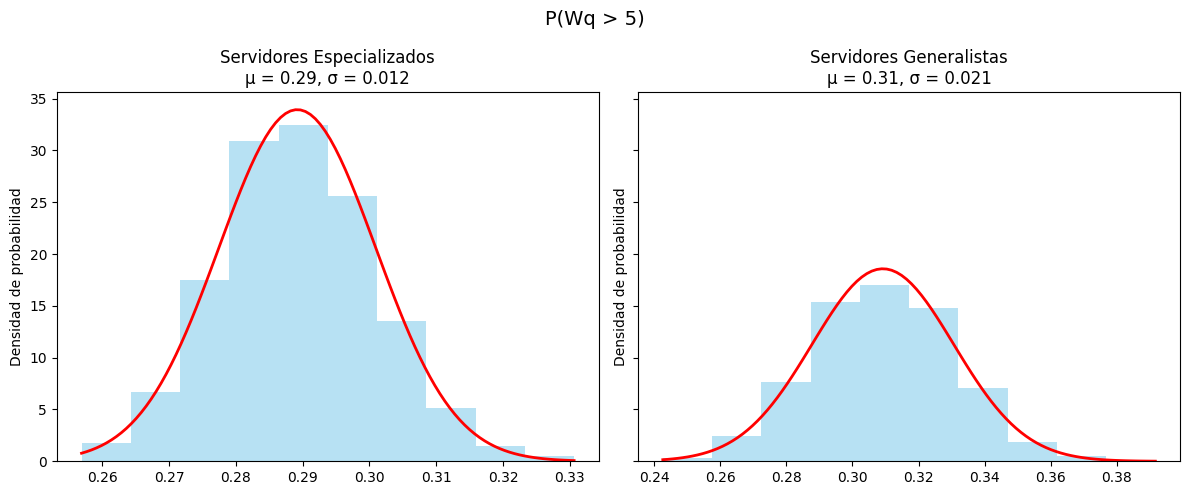
\includegraphics[width=0.95\textwidth]{images/PWqovertk.png}
    \caption{Histograma de la probabilidad de superar el umbral de 5 minutos de espera}
    \label{fig:probabilidad}
\end{figure}


\begin{figure}[H]
    \centering
    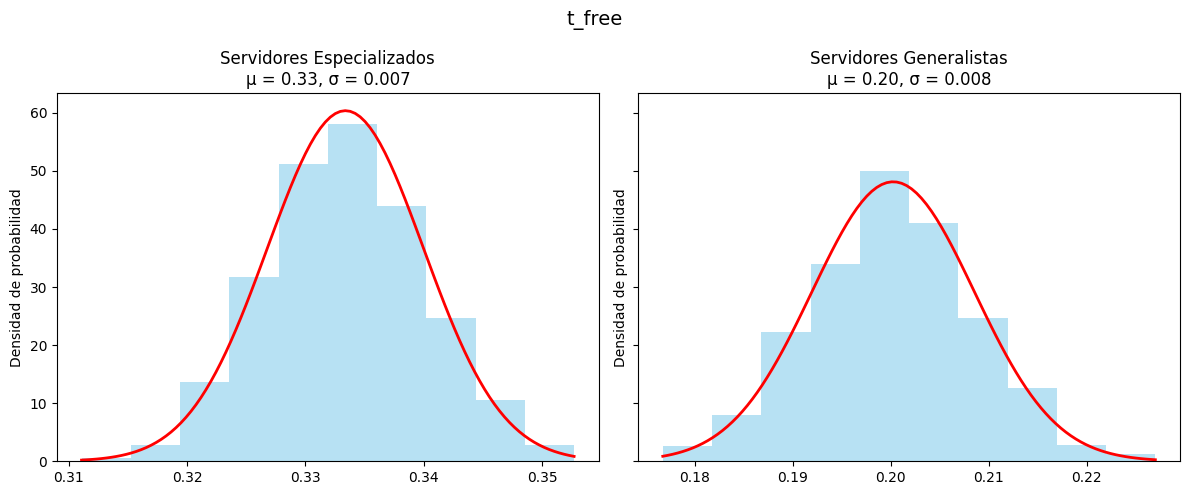
\includegraphics[width=0.95\textwidth]{images/tfree.png}
    \caption{Histograma de la tasa de tiempo inactivo de los servidores}
    \label{fig:inactividad}
\end{figure}

\subsection{Interpretación de los resultados}

\begin{itemize}
    \item Al seguir una estrategia generalista, aunque se distribuye la carga entre dos servidores, el tiempo de servicio por cliente aumenta debido
    a la reducci\'on de la especialización. Por tango, aumenta la congestión del sistema y el tiempo de espera de los usuario.
    \item La probabilidad de retrasos críticos no difiere significativamente, debido a que la distribución exponencial mitiga los efectos de las diferencias en las probabilidades de cola larga.
    \item En el sistema especializado, los servidores no pueden redistribuir la carga. Si una cola está vacía, su servidor permanece inactivo aunque haya demanda en la otra cola, por tanto tiene un peor uso de recursos.
\end{itemize}

\subsection{Hipótesis extraídas}

\subsubsection{Hipótesis 1: Mayor congestión de clientes en sistema generalista}
\begin{itemize}
    \item \textbf{Hipótesis nula:} $H_0: \mu_{\text{propuesto}} \leq \mu_{\text{actual}}$ 
    \item \textbf{Hipótesis alternativa:} $H_1: \mu_{\text{propuesto}} > \mu_{\text{actual}}$ 
\end{itemize}

\subsubsection{Hipótesis 2: Mayor tiempo de espera en sistema generalista}
\begin{itemize}
    \item \textbf{Hipótesis nula:} $H_0: W_{\text{propuesto}} \leq W_{\text{actual}}$ 
    \item \textbf{Hipótesis alternativa:} $H_1: W_{\text{propuesto}} > W_{\text{actual}}$ 
\end{itemize}

\subsubsection{Hipótesis 3: Similar probabilidad de retrasos críticos}
\begin{itemize}
    \item \textbf{Hipótesis nula:} $H_0: p_{\text{actual}} = p_{\text{propuesto}}$ 
    \item \textbf{Hipótesis alternativa:} $H_1: p_{\text{actual}} \neq p_{\text{propuesto}}$ 
\end{itemize}


\subsubsection{Hipótesis 4: Mayor inactividad en sistema especializado}
\begin{itemize}
    \item \textbf{Hipótesis nula:} $H_0: I_{\text{actual}} \leq I_{\text{propuesto}}$ 
    \item \textbf{Hipótesis alternativa:} $H_1: I_{\text{actual}} > I_{\text{propuesto}}$ 
\end{itemize}

\subsection{Pruebas de Hipótesis}

Se realiz\'o un test t-student para cada hipótesis, en todos los casos se 
obtuvieron p-values muy cercanos a 0, así que en todos los casos
se rechaza la hipótesis nula. Se puede asegurar que hay diferencias significativas
en la media de cada variable para las dos estrategias.

\chapter{Modelo matemático}


\section{Descripción del modelo}

Consideramos dos sistemas de colas diferentes bajo teoría de colas markovianas, descritas detalladamente en \cite{queue}. Para ambos sistemas asumimos 
procesos Poisson de llegada con tasa $\lambda$ y servicio con tasa $\mu$. Definimos:
\begin{itemize}
    \item $\rho = \frac{\lambda}{c\mu}$ (intensidad de tráfico, $c$ cantidad de servidores en paralelo)
    \item $L$: Número promedio de clientes en el sistema
    \item $L_q$: Número promedio en cola
    \item $W_q$: Tiempo promedio en cola
\end{itemize}

\subsection{Sistema Actual (Dos Colas M/M/1)}

Para cada servidor simple independiente:
\begin{itemize}
    \item $L = \frac{\lambda}{\mu - \lambda}$
    \item $W_q = \frac{\rho}{\mu - \lambda}$
    \item $P(W_q > t) = \rho e^{-(\mu - \lambda)t}$
    \item $P_{free} = 1 - \rho$
\end{itemize}

\subsection{Sistema Propuesto (Una Cola M/M/2)}
Para el sistema conjunto de los dos servidores en paralelo:
\begin{itemize}
    \item 
    $P_0 = \left[\sum_{k=0}^{1}\frac{(2\rho)^k}{k!} + \frac{(2\rho)^2}{2!(1-\rho)}\right]^{-1}$
    
    \item $L_q = \frac{(2\rho)^2\rho}{2!(1-\rho)^2}P_0$
    
    \item $L = \frac{\lambda}{\mu} + L_q$
    
    \item $W_q = \frac{L_q}{\lambda}$
    
    \item $P(W_q > t) = \frac{2\rho e^{-2\mu(1-\rho)t}}{2 - \rho}P_0$
    
    \item $P_{\text{free}} = 1 - \rho$ \\
\end{itemize}


\section{Supuestos y restricciones}
\begin{itemize}
    \item \textbf{Política FIFO:} Clientes son atendidos en orden de llegada
    \item \textbf{Independencia:} Llegadas y servicios son procesos independientes
    \item \textbf{Uniformidad:} Llegadas y servicios tienen la misma tasa para ambos sistemas y ambos servicios (valores de entrada del problema específico)
    \item \textbf{Espacio infinito:} Capacidad ilimitada en las colas
    \item \textbf{Homogeneidad:} Tasa de servicio constante en el tiempo
\end{itemize}



\section{Comparación de resultados}
\begin{table}[h]
\centering
\caption{Resultados Teóricos vs. Experimentales}
\begin{tabular}{lccccc}
\toprule
\textbf{Métrica} & \multicolumn{2}{c}{\textbf{Sistema actual ($\lambda = 20$, $\mu = 30$)}} & \multicolumn{2}{c}{\textbf{Sistema propuesto ($\lambda = 40$, $\mu = 25$)}} \\
 & Teórico & Experimental & Teórico & Experimental \\
\midrule
Clientes en el sistema & 4.00 & 3.99 & 4.44 & 4.44 \\
Tiempo en cola (min) & 4.00 & 3.99 & 4.27 & 4.26 \\
Prob. de retraso crítico & 0.2895 & 0.29 & 0.3089 & 0.31 \\
Tiempo inactivo (\%) & 33 & 33 & 20 & 20 \\
\bottomrule
\end{tabular}
\end{table}

Los resultados experimentales coinciden con las predicciones teóricas, confirmando la validez de los supuestos markovianos. 
Se concluye que ambos enfoques proveen una base sólida para la toma de decisiones operativas.

\chapter{Conclusiones}


\begin{itemize}
    \item[1.] Servidores especializados provocan bloqueo parcial del sistema debido a las
    colas separadas, lo que lleva a una subutilización de recursos.
    \item[2.] Servidores generalistas son más lentos debido a la falta de especialización,
    provocando una peor experiencia de usuario.
\end{itemize}


\begin{thebibliography}{9}
    \bibitem{queue} SABATER, J. P. G. Aplicando Teoría de Colas en Dirección de Operaciones. [S.l.]:
    Grupo ROGLE, Departamento de Organización de Empresas, Universidad Politécnica
    de Valencia, 2015/2016.
 
\end{thebibliography}




\end{document}
